

\subsection{Client Side Data Buffering, Statistics, and Real Time Plotting}
First the ring buffer collects sensor samples from the sensor thread and then delivers them to the server thread. On the GUI (client) side, a similar mechanism is needed: incoming samples must be stored, organized per sensor, and then used for plotting and statistics. This section explains all data structures and functions responsible for this task.

\subsubsection{Incoming Data - The Network Packet}
Every sample that arrives over TCP is a packed structure called net\_packet\_t:
    \begin{minted}[bgcolor = lightgray, tabsize = 4, breaklines ]{c}
    typedef struct __attribute__((packed)) {
        int32_t sid;      /* sensor ID: 1=Temp, 2=ADC0, 3=ADC1, 4=Switch, 5=PushBtn */
        int32_t svalue;   /* raw sensor value (integer) */
        int64_t ts;       /* timestamp in microseconds from server start */
    } net_packet_t;
\end{minted}

This structure is exactly 16 bytes because this \texttt{\_attribute\_((packed))} directive that it removes any padding between fields. With identifying which sensor produces sample by \texttt{sid} filed, then the \texttt{svalue} holds raw measurement and \texttt{ts} is the timestamp in microseconds assigned by the server's \texttt{GetElapsedTime()} function.

Network thread receives the raw bytes from the TCP socket and it is going to check whether at least \texttt{sizeof(net\_packet\_t)} bytes are available, then it is going to extracts one packet and calls buffer\_add\_sample(pkt.sid, pkt.svalue, pkt.ts) to store the sample in the correct per sensor buffer.

\begin{minted}[bgcolor = lightgray, tabsize = 4, breaklines]{c}
	typedef struct {
    double   values[MAX_SAMPLES];    /* sensor values (converted to double) */
    int64_t  ts_us[MAX_SAMPLES];     /* timestamps in microseconds */
    int      count;                  /* number of stored samples */
    int      oldest_idx;             /* index of oldest sample (when full) */
    int64_t  start_time_us;          /* timestamp of the very first sample */
    pthread_mutex_t lock;            /* protects concurrent access */
	} sensor_buffer_t;
\end{minted}
The constant \texttt{MAX\_SAMPLES} is set to 2000 that means each sensor can only store up to 2000 data points before older values are overwritten. Thers is \texttt{count} filed which is showing  how many samples have been added so far. As long as count < MAX\_SAMPLES, new samples are appended at index count. Once the \texttt{count == MAX\_SAMPLES}, the buffer becomes circular it means buffer is full: new samples overwrite the entry at oldest\_idx, which is then incremented modulo the buffer size.
The start\_time\_us field stores the timestamp of the first sample for that sensor and all the other which is coming later subsequent timestamps are plotted relative to this value, so the x-axis starts near zero.
The pthread\_mutex\_t responsible for lock ensures thread safety. Since the network thread (calling buffer\_add\_sample) and the GTK main thread (calling buffer\_get\_copy and buffer\_stats) run concurrently, the mutex is trying to avoid simultaneous access to the buffer.

\begin{minted}[bgcolor = lightgray, tabsize = 4, breaklines]{c}
sensor_buffer_t buf[MAX_SENSORS + 1];   /* buf[1]..buf[5], index 0 unused */
\end{minted}

\begin{figure}[H]
\centering 
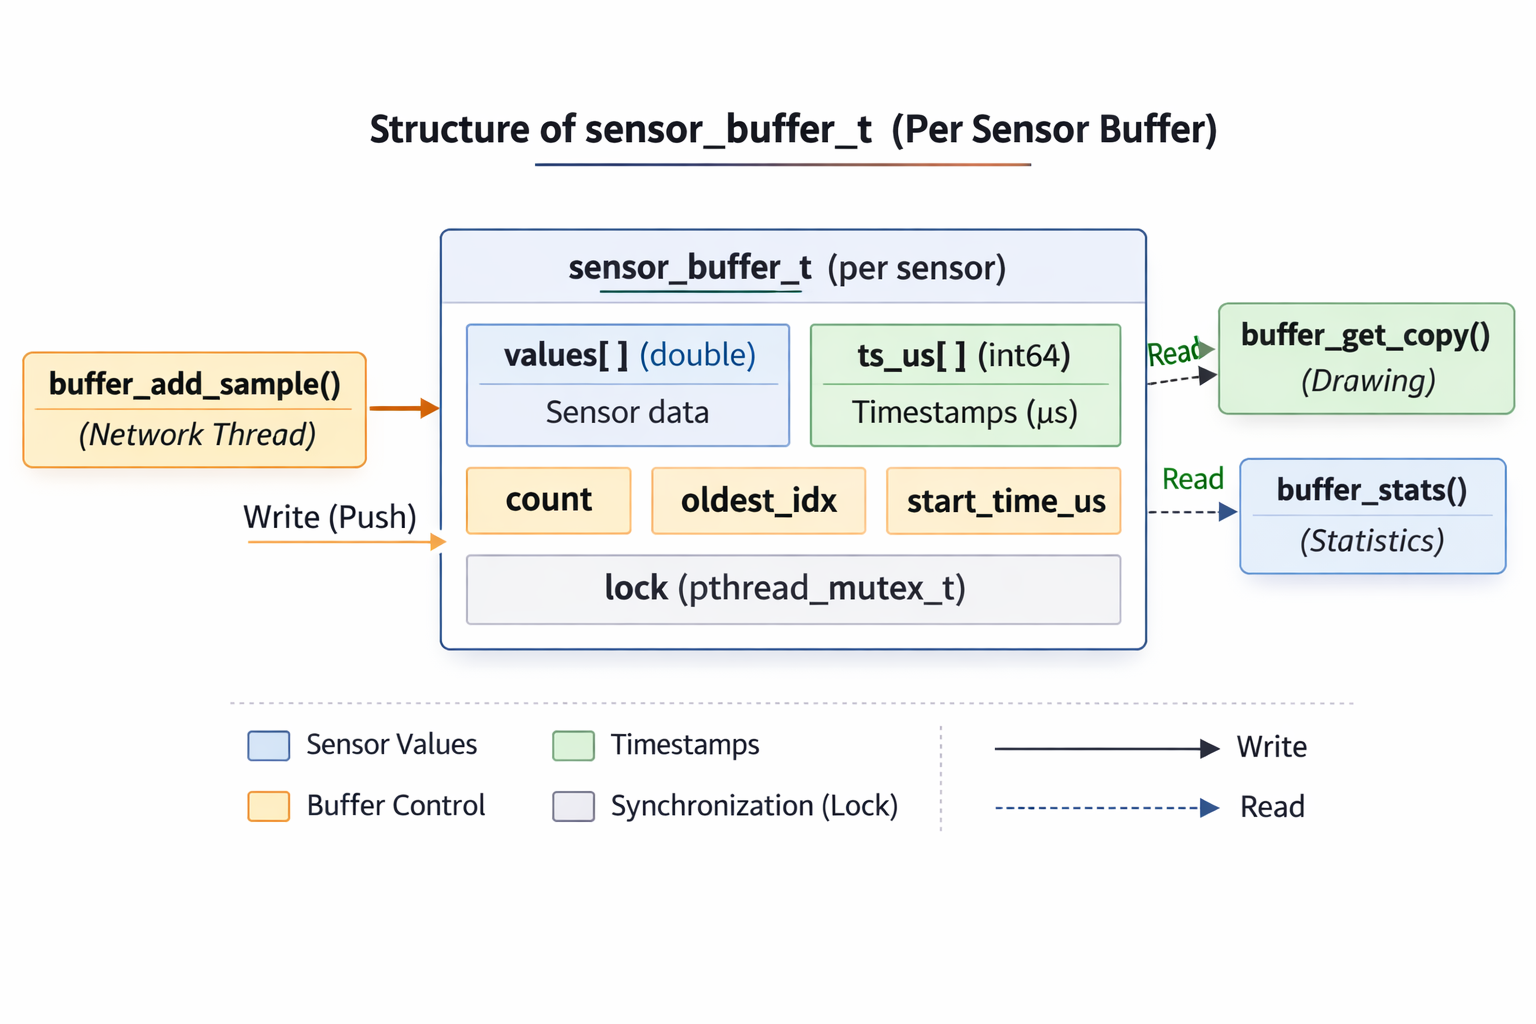
\includegraphics[width = 0.9\textwidth, trim = 0cm 2cm 0cm 0cm, clip]{media/imageRezaGUI1.png}
\caption{Structure of sensor\_buffer\_t}
\label{fig-guireza1}
\end{figure}

\subsubsection{Buffer Initialization \texttt{buffer\_init}}
\begin{minted}[bgcolor = lightgray, tabsize = 4, breaklines]{c}
static void buffer_init(int sid) {
    if (sid < 1 || sid > MAX_SENSORS) return;
    sensor_buffer_t *b = &g_app.buf[sid];
    pthread_mutex_init(&b->lock, NULL);
    b->count = 0;
    b->oldest_idx = 0;
    b->start_time_us = 0;
}
\end{minted}
This function is called once for each sensor (sid = 1 to 5) during the GUI startup in build\_ui(). It initializes the POSIX mutex and sets count, oldest\_idx, and start\_time\_us to zero, which means the buffer starts empty and ready to receive samples.

\subsubsection{Adding a sample \texttt{buffer\_add\_sample}}
\begin{minted}[bgcolor = lightgray, tabsize = 4, breaklines]{c}
static void buffer_add_sample(int sid, int value, int64_t ts_us) {
    if (sid < 1 || sid > MAX_SENSORS) return;
    sensor_buffer_t *b = &g_app.buf[sid];
    pthread_mutex_lock(&b->lock);

    if (b->count == 0) b->start_time_us = ts_us;
    if (ts_us > g_app.last_data_time_us)
        g_app.last_data_time_us = ts_us;

    if (b->count < MAX_SAMPLES) {
        int idx = b->count++;
        b->values[idx] = (double)value;
        b->ts_us[idx]  = ts_us;
    } else {
        int idx = b->oldest_idx;
        b->values[idx] = (double)value;
        b->ts_us[idx]  = ts_us;
        b->oldest_idx  = (b->oldest_idx + 1) % MAX_SAMPLES;
    }

    pthread_mutex_unlock(&b->lock);
}
\end{minted}
This function is the producer of the client side buffer; it is called by the network thread every time a net\_packet\_t is successfully extracted from the TCP stream.

Step by step: 
\begin{enumerate}
\item	Guard check: if sid is out of range (not 1–5), the function returns immediately.
\item	Lock the mutex: prevents the drawing thread from reading the buffer at the same time.
\item	First sample handling: if this is the very first sample (count == 0), the timestamp is saved as start\_time\_us. This becomes the reference point (time zero) for the x axis.
\item	Global timestamp tracking: last\_data\_time\_us is updated to the newest timestamp across all sensors, which is later used to determine the right edge of the time window in the chart.
\item	Buffer not yet full (count < MAX\_SAMPLES): the sample can still to be written at position count, and then count is incremented.
\item	Buffer full (count == MAX\_SAMPLES): the sample will overwrites the oldest entry at oldest\_idx, and oldest\_idx is going to advance by one with wrap around (\% MAX\_SAMPLES). This is the same circular buffer principle as the server ring buffer.
\item	Unlock the mutex.
\end{enumerate}

\subsubsection{Reading Samples for Plotting - buffer\_get\_copy}
\begin{minted}[bgcolor = lightgray, tabsize = 4, breaklines]{c}
static int buffer_get_copy(int sid, double *x_ms, double *y, int max_len) {
    if (sid < 1 || sid > MAX_SENSORS) return 0;
    sensor_buffer_t *b = &g_app.buf[sid];
    pthread_mutex_lock(&b->lock);

    if (b->count == 0) { pthread_mutex_unlock(&b->lock); return 0; }
    int n = (b->count < max_len) ? b->count : max_len;

    if (b->count < MAX_SAMPLES) {
        for (int i = 0; i < n; ++i) {
            x_ms[i] = (double)(b->ts_us[i] - b->start_time_us) / 1000.0;
            y[i]    = b->values[i];
        }
    } else {
        for (int i = 0; i < n; ++i) {
            int idx = (b->oldest_idx + i) % MAX_SAMPLES;
            x_ms[i] = (double)(b->ts_us[idx] - b->start_time_us) / 1000.0;
            y[i]    = b->values[idx];
        }
    }

    pthread_mutex_unlock(&b->lock);
    return n;
}
\end{minted}

This is the consumer of the client side buffer; it is called by the drawing function every time the chart needs to be redrawn.
Key points:
\begin{enumerate}
\item It locks the mutex, copies the data into the caller's arrays (x\_ms and y), and unlocks immediately, this minimizes the time the mutex is held, keeping the network thread responsive.
\item Timestamp conversion: the raw microsecond timestamps are converted to milliseconds relative to start\_time\_us using (ts\_us[i] - start\_time\_us) / 1000.0. It shows that the x-axis of chart always start from near zero.
\item Buffer not full (count < MAX\_SAMPLES): data is stored sequentially starting from index 0, so the loop reads indices 0 to n−1 directly.
\item Buffer full: data is read starting from oldest\_idx (the oldest sample), wrapping around with modulo. This guarantees that output should always in somehow order which from oldest to newest.
\item The function returns n, the number of copied samples.
\end{enumerate}


\subsubsection{Computing Statistics - \texttt{buffer\_stats}}
\begin{minted}[bgcolor = lightgray, tabsize = 4, breaklines]{c}
static int buffer_stats(int sid, double *minv, double *maxv,
                        double *avg, int *count) {
    if (sid < 1 || sid > MAX_SENSORS) return 0;
    sensor_buffer_t *b = &g_app.buf[sid];
    pthread_mutex_lock(&b->lock);

    if (b->count == 0) { pthread_mutex_unlock(&b->lock); return 0; }
    double mn = b->values[0], mx = b->values[0], sum = 0.0;
    for (int i = 0; i < b->count; ++i) {
        double v = b->values[i];
        if (v < mn) mn = v;
        if (v > mx) mx = v;
        sum += v;
    }
    *minv = mn;  *maxv = mx;
    *avg  = sum / b->count;
    *count = b->count;

    pthread_mutex_unlock(&b->lock);
    return 1;
}
\end{minted}
This function is computing the minimum, maximum, and average of all stored samples which are for a given sensor. It is called by \texttt{update\_stats\_box()} every 50 ms (the GUI refresh interval). The result is displayed as a formatted line in the ‘Statistics’ panel below the chart. For example:
\begin{center}
\begin{minted}[bgcolor = lightgray, tabsize = 4, breaklines]{text}
SID 1 Temperature (°C) | Min: 23.5 Max: 26.1 Avg: 24.8 (n=1500)
\end{minted}
\end{center}

The function trying to process all stored values in a single pass, then tracking the running minimum, maximum, and sum. Dividing the sum by count yields the arithmetic mean. If the buffer is empty, the function returns 0 and the sensor is omitted from the statistics display.

\subsubsection{Displaying Statistics - \texttt{update\_stats\_box}}
The function \texttt{update\_stats\_box()} is called periodically by the GUI refresh
timer. It performs two steps:

\begin{enumerate}
    \item \textbf{Clear old labels:} It is responsible to remove all child widgets
    from \texttt{g\_app.stats\_box} (the vertical box inside the Statistics frame),
    and trying to prevent the panel from accumulating outdated entries.

    \item \textbf{Rebuild for each active sensor:} For every sensor where
    \texttt{sensor\_enabled[sid]} is true, it calls \texttt{buffer\_stats()} to get
    the current min, max, average, and count, it formats the result into a line using
    \texttt{snprintf}, and then it creates a new GTK label with monospace markup, and
    adds it to the stats box.
\end{enumerate}

This approach rebuilds the statistics display from scratch every refresh cycle, which
is simple and avoids the need to track individual label widgets per sensor.

\subsubsection{Real Time Chart - \texttt{on\_draw\_chart}}
The \texttt{on\_draw\_chart()} function is the Cairo drawing callback which is connected
to the \texttt{GtkDrawingArea}. GTK calls it automatically whenever
\texttt{gtk\_widget\_queue\_draw()} is triggered, which occurs every 50\,ms via the
\texttt{ui\_update\_cb} timer.

The drawing process has five stages:

\begin{enumerate}
    \item \textbf{Stage 1-Background and grid:} The function clears the drawing area
    which is using a dark background color (\texttt{rgb(0.06, 0.08, 0.10)}) and it is
    going to draws five horizontal grid lines plus the X and Y axes in gray.

    \item \textbf{Stage 2-Determine data range:} A first loop iterates over all enabled
    sensors, calls \texttt{buffer\_get\_copy()} for each, and then it scans the returned
    values to determine the global minimum and maximum for both the time (x-axis) and
    value (y-axis). If there is no sensor has data, the function displays
    ``Waiting for data\ldots'' and returns.

    \item \textbf{Stage 3-Time window and y-axis scaling:} The user-selected time window
    (\texttt{time\_range\_seconds}, e.g., 5 seconds = 5000\,ms) which it defines the
    visible data range. The right edge of the window (\texttt{t\_max}) is set to the
    latest timestamp, and the left edge (\texttt{t\_min}) is
    \texttt{t\_max}~\(-\)~\texttt{time\_window\_ms}. A 10\% padding is added above and
    below the y-range so curves do not touch the borders.

    \item \textbf{Stage 4-Draw sensor curves:} A second loop iterates over all enabled
    sensors again. For each sensor, \texttt{buffer\_get\_copy()} provides the
    (time, value) arrays. Each sensor has a unique color defined in the
    \texttt{g\_sensors} table (e.g.\ temperature = light blue, ADC0 = red). The code
    maps each data point from data coordinates to pixel coordinates using:
    
    \begin{minted}[bgcolor = lightgray, tabsize = 4, breaklines]{text}
pixel_x = margin_left + ((time_ms - t_min) / t_range) * plot_width
pixel_y = margin_top + plot_height - ((value - y_min) / y_range) * plot_height
\end{minted}

Points outside the time window are skipped, and the curve is drawn as a polyline using cairo\_move\_to(), cairo\_line\_to(), and cairo\_stroke().

\item \textbf{Stage 5-Axis labels and title:} The y-axis shows six evenly spaced value ticks, the x-axis shows six evenly spaced time ticks (in milliseconds), and a title at the top displays the current time window (for example, “Real-Time Sensor Data - 1200.0 to 6200.0 ms”).
\end{enumerate}



\begin{figure}[H]
\centering 
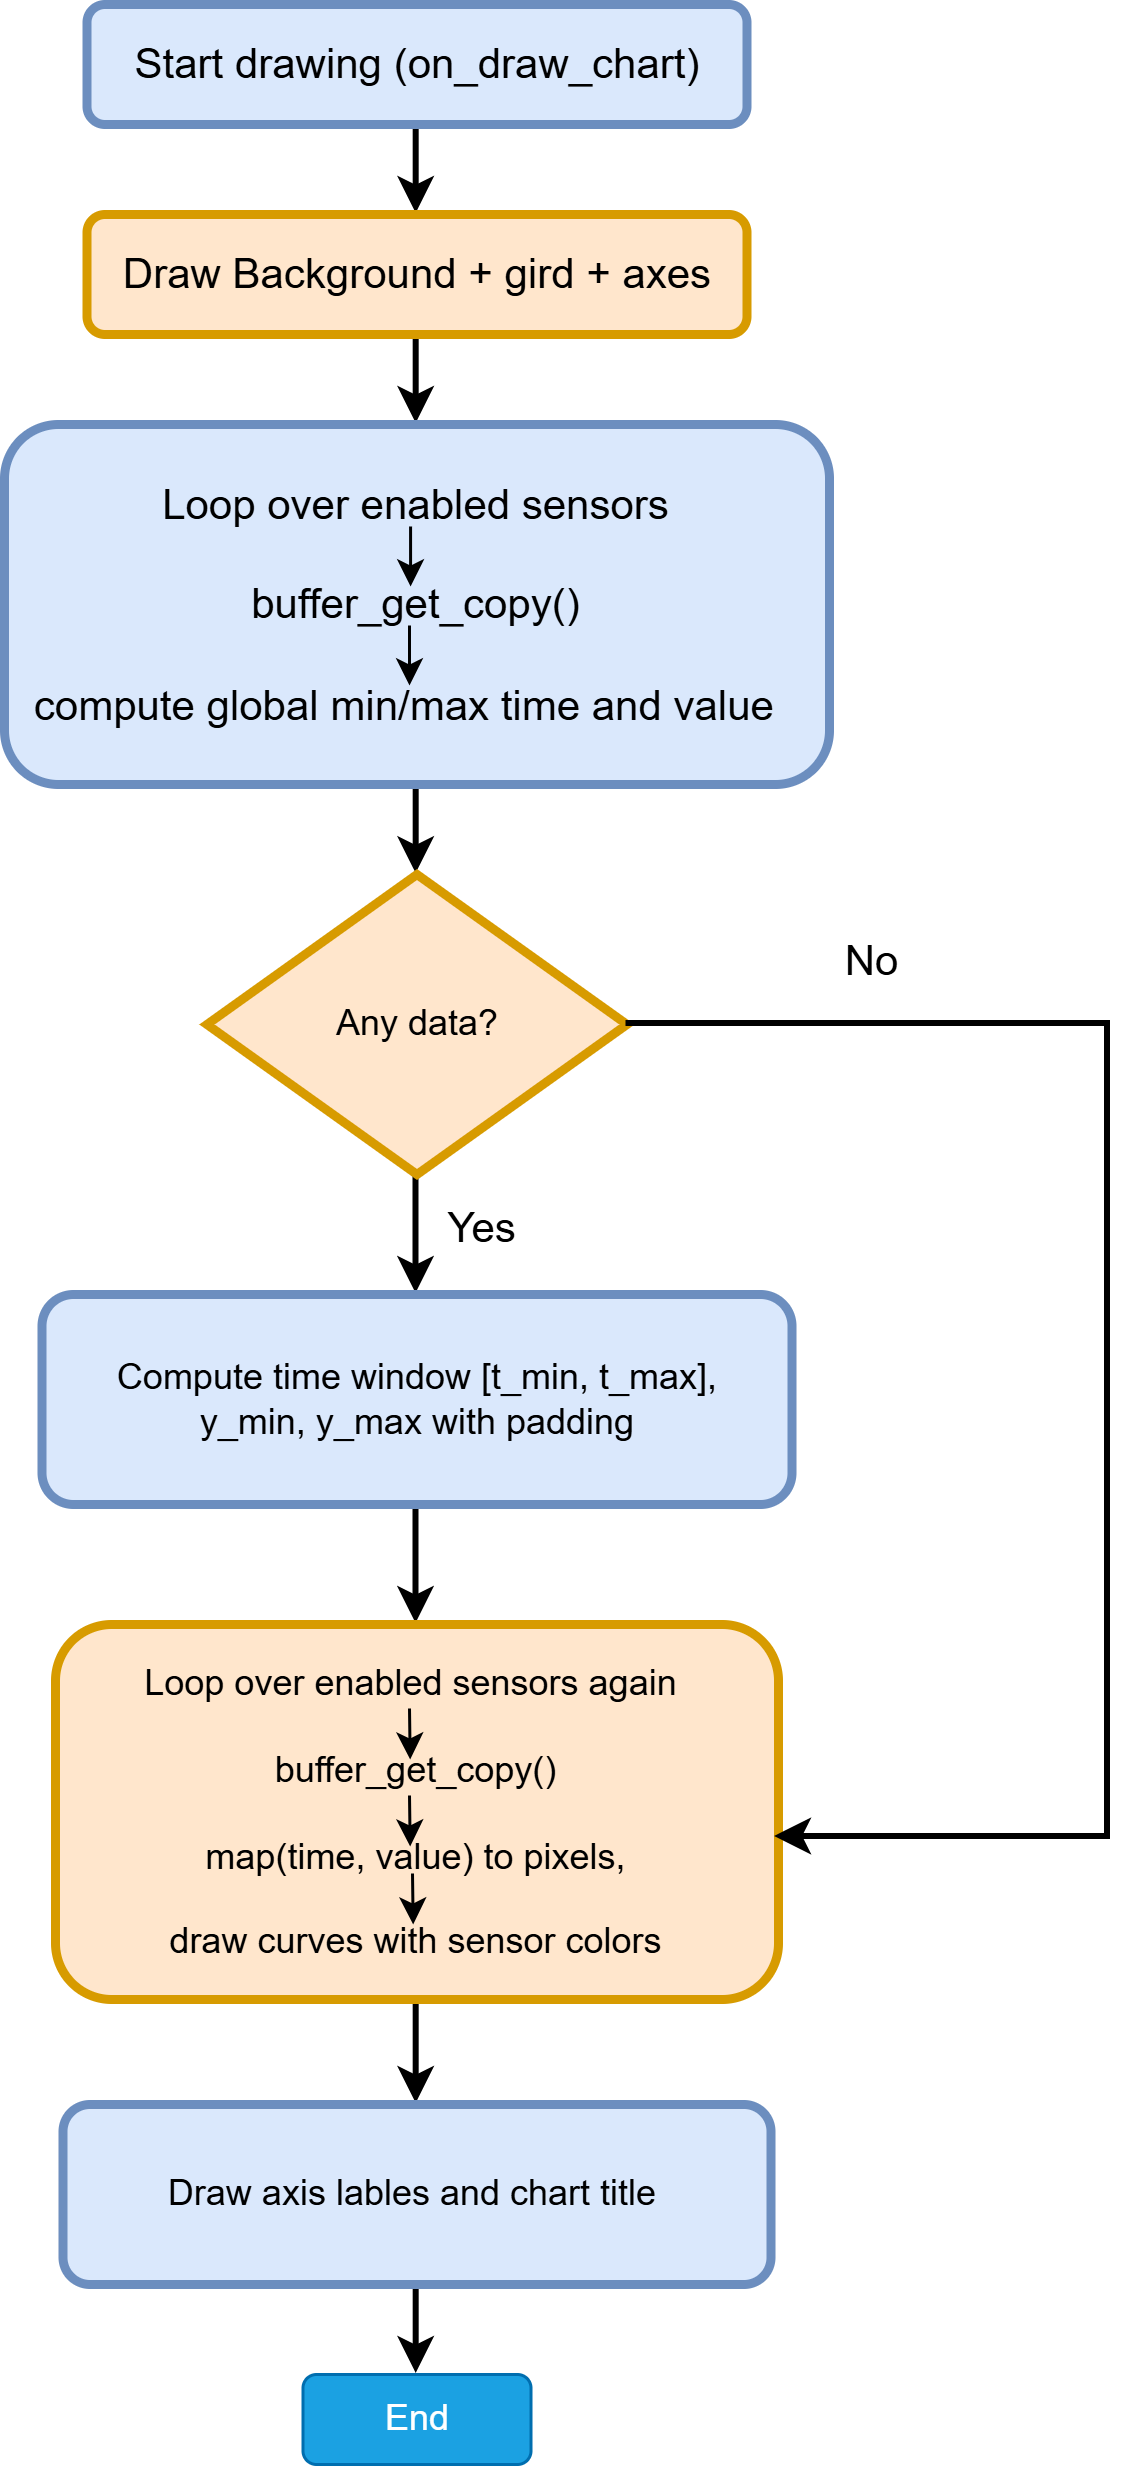
\includegraphics[scale = 0.8]{media/imageRezaGUI2.png}
\caption{Drawing pipeline inside \texttt{on\_draw\_chart()}}
\label{fig-rezagui2}
\end{figure}

\subsubsection{Sensor Visibility and Time Window Control}
Two user controls directly affect the chart and statistics:

\begin{itemize}
    \item \textbf{Visible Sensors checkboxes:} each sensor has a \texttt{GtkCheckButton}.
    When the user toggles it, the \texttt{on\_sensor\_toggled()} callback sets
    \texttt{g\_app.sensor\_enabled[sid]} to true or false and triggers a redraw. Just
    the enabled sensors are included in the global min/max calculation, plotting, and
    statistics panel display.

    \item \textbf{Display Window slider:} A horizontal \texttt{GtkScale} lets the user
    select how many seconds of data are visible (1 to 5 seconds). 
\end{itemize}
The \texttt{on\_time\_range\_changed()} callback updates \texttt{g\_app.time\_range\_seconds} and also the label text (for example, ‘5 sec’), then it triggers a redraw. With a larger window shows more history but there will be less detail. So a smaller window zooms in on the latest samples.

\subsubsection{Periodic Refresh - \texttt{ui\_update\_cb}}
\begin{minted}[bgcolor = lightgray, tabsize = 4, breaklines]{c}
static gboolean ui_update_cb(gpointer data) {
    if (g_app.should_close) return FALSE;
    /* update status label based on connection state */
    gtk_widget_queue_draw(g_app.drawing_area);
    update_stats_box();
    return TRUE;
}
\end{minted}
This timer callback is registered once in main() with a period of UPDATE\_INTERVAL\_MS = 50 ms, meaning the chart and statistics refresh at approximately 20 frames per second. It calls \texttt{gtk\_widget\_queue\_draw()}, which tells GTK to invoke \texttt{on\_draw\_chart()} on the next main loop iteration, and \texttt{update\_stats\_box()} to rebuild the statistics panel. Returning \texttt{TRUE} keeps the timer repeating; returning \texttt{FALSE} (when the window is closing) stops it.

\subsubsection{Connection to the Server Side Ring Buffer}
This client-side buffering is the second stage of the overall data pipeline in the
Measurement Network Gateway:

\begin{itemize}
    \item \textbf{Server ring buffer (your ring buffer chapter):} the sensor thread
    pushes timestamped (\texttt{sid}, \texttt{ts}, \texttt{svalue}) entries; the server
    thread pops them and packs them into TCP packets.

    \item \textbf{TCP transport:} packets travel from the server to the GUI client as
    raw \texttt{net\_packet\_t} bytes.

    \item \textbf{Client per-sensor buffers (this section):} incoming packets are sorted
    by \texttt{sid} into five separate circular buffers, converted to doubles, and made
    available for plotting and statistics.
\end{itemize}

The server ring buffer holds all five sensors mixed together in a single FIFO queue,
while the client separates them into individual buffers so each sensor can be plotted
and analyzed independently.

\begin{figure}[H]
\centering 
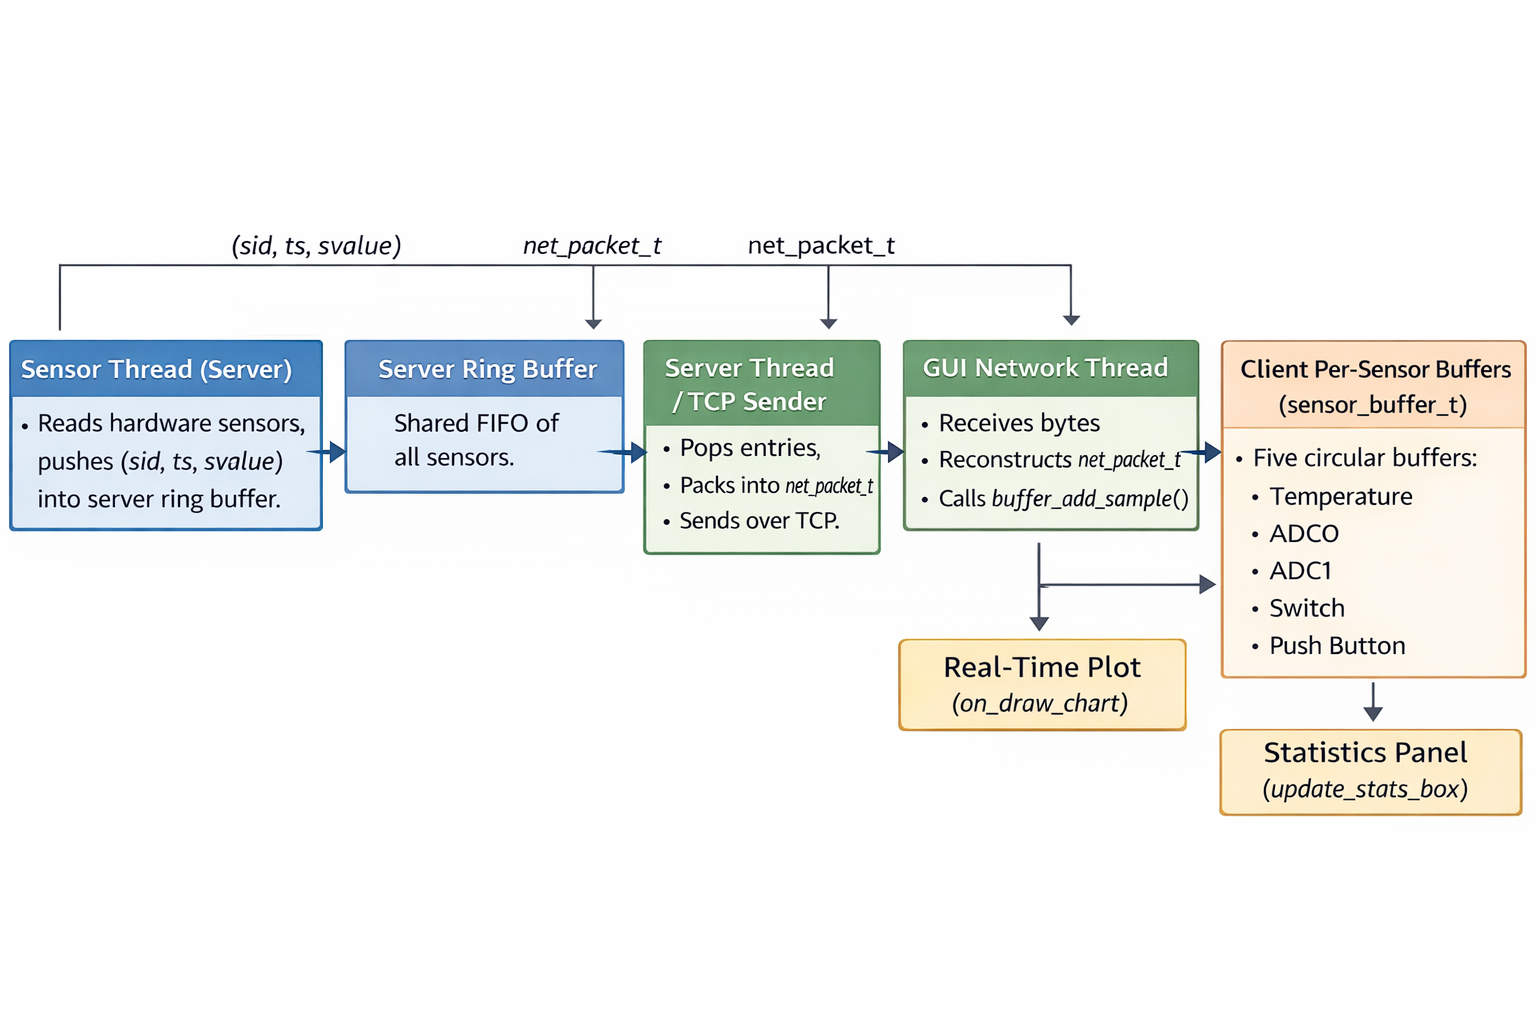
\includegraphics[width = 0.85\textwidth]{media/imageRezaGUI3.png}
\caption{Data flow from server ring buffer to GUI buffers}
\label{fig-rezagui3}
\end{figure}



\section{Requirement Compliance and Verification}
This section discusses the compliance of requirements for the application and GUI built by Mohammad Mahdi Mohammadi, Mohammad Reza Rahimi and Akshay Vastrad. 
\subsection{Compliance Summary}
The Measurement Network Gateway system has been developed and verified against a total of 24 specified requirements covering Functional, Design, RAMS, and Test categories.
\begin{table}[h!]
    \centering
    \caption{Requirements Compliance Summary}
    \begin{tabular}{|l|c|c|}
        \hline
        \textbf{Category} & \textbf{Total Requirements} & \textbf{Implemented}\\
        \hline
        Functional & 12 & 12 \\
        Design     & 5  & 5  \\
        RAMS       & 4  & 4  \\
        Test       & 3  & 3  \\
        \hline
        \textbf{TOTAL} & \textbf{24} & \textbf{24} \\
        \hline
    \end{tabular}
    \label{tab:requirements_compliance}
\end{table}

All 24 system requirements have been fully implemented and verified. No open compliance gaps remain.



\subsection{Requirements Traceability Matrix}

\begin{table}[h!]
    \centering
    \label{tab:req_traceability}
    \small
    \begin{tabularx}{\linewidth}{|l|X|X|l|}
        \hline
        \textbf{Req ID} & \textbf{Requirement Description} & \textbf{Technical Implementation} & \textbf{Verification Method} \\
        \hline
        REQ-1  & Multi-sensor TCP gateway              & Sensor + Server threads, Ring Buffer, TCP port 50012          & Integration test         \\
        \hline
        REQ-2  & Precision RTD temperature acquisition & PT100 + MAX31865, \texttt{TempRead()}, \texttt{sid\_temp}     & Sensor validation test   \\
        \hline
        REQ-3  & Dual ADC signal capture               & PmodAD1 (ADC0/ADC1), \texttt{GetADC()}, \texttt{sid\_adc0/1} & Signal injection test    \\
        \hline
        REQ-4  & Digital switch acquisition            & ZedBoard 8-bit DIP, \texttt{ReadSwitch()}                     & Functional test          \\
        \hline
        REQ-5  & Pushbutton acquisition                & ZedBoard 5 buttons, \texttt{ReadButton()}                     & Functional test          \\
        \hline
        REQ-6  & Configurable sampling rates           & Per-sensor Hz config, \texttt{period\_us = 1M/Hz}             & Timing verification      \\
        \hline
        REQ-7  & Selectable sensor activation          & Rate=0 disables sensor, conditional sampling                  & Configuration test       \\
        \hline
        REQ-8  & Timestamped measurements              & \texttt{CLOCK\_MONOTONIC}, 1\,\textmu s resolution            & Time accuracy validation \\
        \hline
        REQ-9  & GUI sensor configuration              & GTK configuration panel                                       & GUI validation           \\
        \hline
        REQ-10 & GUI sampling rate configuration       & Per-sensor Hz input fields                                    & GUI validation           \\
        \hline
        REQ-11 & GUI text data display                 & Live table with real-time updates                             & Runtime test             \\
        \hline
        REQ-12 & GUI dual-signal plotting              & Cairo-based dual-channel charts                               & Visual verification      \\
        \hline
    \end{tabularx}
    \caption{Functional Requirements (REQ-1 \rightarrow REQ-12)}
\end{table}


\begin{table}[h!]
    \centering
    \label{tab:design_traceability}
    \small
    \begin{tabularx}{\linewidth}{|l|X|X|l|}
        \hline
        \textbf{Req ID} & \textbf{Requirement} & \textbf{Implementation} & \textbf{Verification} \\
        \hline
        REQ-13 & Embedded Linux platform       & Zynq-7000 ZedBoard, ARM Cortex-A9, PetaLinux        & Platform validation  \\
        \hline
        REQ-14 & Multithreaded architecture    & Two POSIX threads with mutex synchronization         & Concurrency test     \\
        \hline
        REQ-15 & GTK-based GUI application     & GTK+3.0, GLib event loop                            & GUI validation       \\
        \hline
        REQ-16 & Binary data protocol          & 16-byte packet structure                            & Protocol inspection  \\
        \hline
        REQ-17 & TCP payload $\leq$ 1500 bytes & $93 \times 16$B packets $= 1488$ bytes               & Network measurement  \\
        \hline
    \end{tabularx}
    \caption{Design Requirements (REQ-13 \rightarrow REQ-17)}
\end{table}




\begin{table}[H]
    \centering
    \label{tab:rams_traceability}
    \small
    \begin{tabularx}{\linewidth}{|l|X|X|l|}
        \hline
        \textbf{Req ID} & \textbf{Requirement} & \textbf{Implementation} & \textbf{Verification} \\
        \hline
        REQ-18 & Controlled startup and shutdown & Thread creation/join, graceful termination                                          & Lifecycle test      \\
        \hline
        REQ-19 & Resource initialization         & \texttt{InitTimer()}, \texttt{InitRingBuffer()}, \texttt{TempPowerUp()}              & Code inspection     \\
        \hline
        REQ-20 & Sensor power-down handling      & \texttt{TempShutdown()} disables MAX31865 VBIAS                                     & Hardware validation \\
        \hline
        REQ-21 & Resource cleanup                & Mutex destroy, socket close, thread join                                            & Shutdown validation \\
        \hline
    \end{tabularx}
    \caption{RAMS Requirements (REQ-18 to REQ-21)}
\end{table}


\begin{table}[h!]
    \centering
    \label{tab:test_traceability}
    \small
    \begin{tabularx}{\linewidth}{|l|X|X|l|}
        \hline
        \textbf{Req ID} & \textbf{Requirement} & \textbf{Implementation} & \textbf{Verification} \\
        \hline
        REQ-22 & Auxiliary digital test inputs      & Switches/buttons used as test signals          & Hardware validation   \\
        \hline
        REQ-23 & Functional testing capability      & Simulation mode with synthetic data            & Mode comparison test  \\
        \hline
        REQ-24 & Timing performance evaluation      & Microsecond timestamps, jitter logging         & Timing analysis       \\
        \hline
    \end{tabularx}
    \caption{Test Requirements (REQ-22 to REQ-24)}
\end{table}


